
\documentclass[12pt]{beamer}
\usepackage{xcolor}
\usepackage{pgf,pgfarrows,pgfnodes,pgfautomata,pgfheaps,pgfshade}
\usetheme{Air}

\DeclareMathOperator*{\argmax}{arg\,max}

\title[CSC349A Numerical Analysis]{CSC349A Numerical Analysis}


\logo{\pgfputat{\pgfxy(-0.5,7.5)}{\pgfbox[center,base]{
\includegraphics[width=1.0cm]{figures/uvic}}}}  
\beamertemplatenavigationsymbolsempty

    \defbeamertemplate{footline}{author and page number}{%
      \usebeamercolor[fg]{page number in head/foot}%
      \usebeamerfont{page number in head/foot}%
      \hspace{1em}\insertshortauthor\hfill%
      \insertpagenumber\,/\,\insertpresentationendpage\kern1em\vskip2pt%
    }
    \setbeamertemplate{footline}[author and page number]{}



\subtitle[Lecture 10]{Lecture 10}
\date[2023]{2023}
\author[R. Little]{Rich Little}
\institute[University of Victoria]{University of Victoria}
%\logo{\includegraphics[scale=.25]{unilogo.pdf}}
\begin{document}
\frame{\maketitle} % <-- generate frame with title


\AtBeginSection[]
{
\begin{frame}<beamer>[allowframebreaks]{Table of Contents}
\tableofcontents[currentsection,currentsubsection, 
    hideothersubsections, 
    sectionstyle=show/shaded,
]
\end{frame}
}


\section{Secant method} 

\begin{frame}{Introduction}
\begin{itemize}
\item{The advantage of the Newton method is that it provides quadratic
convergence.}
\item{One disadvantage is that it requires knowledge of the
derivative $f'(x)$.}
\item{In many applications the derivative might not be
known or impossible to derive analytically through calculus.}
\item{In this case it is possible to use a discrete approximation to the
derivative. One such approximation is used in the {\it Secant}
method.}
\end{itemize}
\end{frame}

\begin{frame}{Secant derivation} 
We can derive the {\it Secant} method starting from the update
equation of the Newton/Raphson method: 
\[
x_{i+1} = x_i - \frac{f(x_i)}{f'(x_i)}
\]
\noindent 
We can approximate $f'(x_i)$ by a finite divided difference: 
\[
f'(x_i) = \lim_{x \rightarrow x_i} \frac{f(x)-f(x_i)}{x-x_i} 
\]
\noindent 
using 
\[
f'(x_i) \approx \frac{f(x_{i-1})-f(x_i)}{x_{i-1} - x_i}
\]
\noindent 
gives: 
\[
x_{i+1} = x_i - \frac{f(x_i)(x_{i-1}-x_i)}{f(x_{i-1}) - f(x_{i})}
\]

%% Notice that the {\it Secant} method requires two initial
%% approximations to the root $x_0$ and $x_1$. 
\end{frame} 


\begin{frame}{Secant Geometry} 
\begin{figure} 
  \centering
  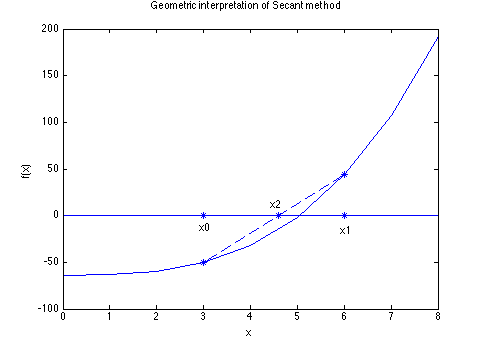
\includegraphics[scale=0.5]{secant}
  \caption{Geometric interpetation of the Secant method for
    root finding.}
  \label{fig:newton}
\end{figure}
\end{frame} 

\begin{frame}{Example of Secant Method} 

Estimate the root of $f(x) = e^{-x} -x$ employing initial guesses of
$x_{-1} = 0$ and $x_0 = 1$. Recall $x_t=0.56714329...$
\vspace{3 in}
\end{frame} 

\begin{frame}{Example of Secant Method continued} 

Estimate the root of $f(x) = e^{-x} -x$ employing initial guesses of
$x_{-1} = 0$ and $x_0 = 1$. The iterative equation can be applied to compute: 

\begin{table}[h]
\begin{tabular}{c|c|c} 
$i$ & $x_i$ & $\varepsilon_t(\%)$ \\ 
\hline 
$-1$ & $0$ & $100$ \\
$0$ & $1$ & $76$ \\ 
$1$ & $0.61270$ & $8.03$ \\
$2$ & $0.56384$ & $0.58$ \\ 
$3$ & $0.56717$ & $0.0048$ \\  
\hline
\end{tabular} 
\end{table} 
\noindent 
Notice that the approach converges on the true root faster than 
{\it Bisection} but slower than {\it Newton}. 
\end{frame} 


\section{Order of convergence of Secant and Bisection} 

\begin{frame}{Order of convergence of the Secant method}
The order of convergence of the Secant method derives from the following limit, 
\begin{equation} 
\lim_{i \rightarrow \infty} \left| \frac{E_{i+1}}{E_iE_{i-1}}\right| = \left| \frac{f''(x_t)}{2f'(x_t)} \right|
\end{equation} 
\noindent 
This gives a relationship {\bf between 3 successive errors}. 
However, this does indicate the {\bf order} $\alpha$ of the Secant method, which requires that the errors of 2 successive approximations be related by 
\begin{equation} 
\lim_{i \rightarrow \infty} \frac{|E_{i+1}|}{|E_i|^{\alpha}} = \lambda, \;\;\; \mbox{for some constant } \lambda 
\end{equation} 
\end{frame} 

\begin{frame}{Secant and Golden Ratio} 
It can be shown in fact that, 
\begin{equation} 
\lim_{i \rightarrow \infty} \left| \frac{E_{i+1}}{E_iE_{i-1}}\right| = \lim_{i \rightarrow \infty} \frac{|E_{i+1}|}{|E_i|^{\alpha}} = \left| \frac{f''(x_t)}{2f'(x_t)} \right|
\end{equation}
where 
\[
\alpha = 1 + \frac{1}{\alpha} \implies \alpha^2 - \alpha -1 = 0 \implies \alpha = \frac{1+\sqrt{5}}{2} \approx 1.618 
\]
\noindent 
which is the {\bf order of the Secant method}. 

\noindent 
{\bf Note:} this value $\alpha$ is known as the ``golden ratio'', and occurs in many places in nature as well as many diverse applications. 
\end{frame} 


\begin{frame}{Bisection convergence} 
An alternate definition of {\bf linear convergence}: 
\[
|E_i| \leq c|E_{i-1}| \mbox{ or } |x_t - x_i| \leq c |x_t - x_{i-1}|
\]
\noindent 
for some constant $c$ such that $0 < c < 1$. 

Applying this inequality recursively gives 
\[
|x_t - x_i| \leq c^{i} |x_t-x_0|
\]
\noindent 
For the Bisection method we had (Handout 8, pg. 2): 
\[
|x_t - x_i| \leq \left( \frac{1}{2}\right)^i \Delta x^0,\mbox{where } \Delta x^{0} = x_u - x_l 
\]
\noindent 
and $[x_l, x_u]$ is the initial interval. This implies linear convergence with the above definition, and $c=\frac{1}{2}$. 
\end{frame} 


\section{The Multiplicity of a Zero} 

\begin{frame}{Introduction} 
If Newton's method converges to a zero $x_t$ of $f(x)$, a necessary
condition for quadratic convergence is that $f'(x_t) \neq 0$ . We now
relate this condition on the derivative of $f(x)$ to the multiplicity
of the zero $x_t$.

\end{frame} 

\begin{frame}{Multiplicity} 

\begin{theorem} 
If $x_t$ is a zero of any analytic function $f(x)$, then there exists a
positive integer $m$ and a function $q(x)$ such that : 

\[
f(x)=(x - x_t)^mq(x),\;\;\mbox{where } \;\; \lim_{x \rightarrow x_t} q(x) \neq 0
\] 
\end{theorem} 

(In particular, if $q(x_t)$ is defined, note that $q(x_t ) \neq 0$.) The
value $m$ is called the {\bf multiplicity} of the zero $x_t$. If $m=1$, then 
$x_t$ is called a {\bf simple zero} of $f(x)$. 
\end{frame} 

\begin{frame}{Example 1} 
Function $f(x) = x^4 + 9.5 x^3 + 18 x^2 - 56x - 160 = (x+4)^3(x-2.5) $ has two zeroes, determine the multiplicity of each.

\vspace{2 in}
\end{frame} 

\begin{frame}{Example 2} 
Let $f(x) = e^x - x - 1$. Since $f(0)=0$, $x_t =0$ is a zero of $f(x)$. What is it's multiplicity?
\vspace{3 in}
\end{frame} 

\begin{frame}{Simple Zero Theorem} 

\begin{theorem} 
Suppose that $f(x)$ and $f'(x)$ are continuous on some interval $[a, b]$, 
and that $x_t \in (a,b)$ and $f(x_t)=0$. Then $x_t$ is a simple zero of $f(x)$ 
if and only if $f'(x_t) \neq 0$. 
\end{theorem} 
\end{frame} 

\begin{frame}{Simple zero - Proof $\Rightarrow$} 

\end{frame} 

\begin{frame}{Simple zero - Proof $\Leftarrow$} 

\end{frame} 


\begin{frame}{Corrolary} 

The following result follows directly from the above Theorem and our 
previous result about the quadratic convergence of Newton's method. 

\begin{block}{Corrolary} 
If Newton’s method converges to a simple zero $x_t$ of $f(x)$, 
then the order of convergence is $2$. 
\end{block} 

In order to determine whether or not Newton’s method converges
quadratically to a zero $x_t$ of $f(x)$, you only need to know whether
the multiplicity of $x_t$ is $1$ or is $\geq 2$. The following result
is more general than the above Theorem, and enables you to determine the
exact multiplicity of a zero.

\end{frame} 


\begin{frame}{Multiplicity and derivatives}

\begin{theorem}

Suppose that $f(x)$ and its first $m$ derivatives are continuous on some
interval $[a,b]$ that contains a zero $x_t$ of $f(x)$. Then the
multiplicity of $x_t$ is $m$ if and only if $f(x_t)= f'(x_t) = f''(x_t) = \dots =
f^{(m-1)}(x_t)=0$ but $f^{(m)}(x_t) \neq 0$.
\end{theorem} 

\end{frame} 

\begin{frame}{Example 3} 
Use the above theorem to show that $f(x) = e^{x} - x - 1$ has root $x_t=0$ of multiplicity 2.
\vspace{3 in}
\end{frame} 

\begin{frame}{Significance of multiplicity} 

\begin{itemize} 
\item Bracketing methods, such as the Bisection method, cannot be used to compute zeros of {\bf even} multiplicity. 

\item Newton's method and the Secant method both converge only linearly (order of convergence is $\alpha = 1$) if the multiplicity $m$ is $\geq 2$. 

\end{itemize} 
\end{frame} 

\begin{frame}{Variant} 

A quadratically convergent algorithm for computing a zero $x_t$ of any
(unknown) multiplicity of a function $f(x)$ is obtained by applying
Newton’s method to the new function.

\[
u(x) = \frac{f(x)}{f'(x)} 
\] 
\noindent 
rather than to $f(x)$. This is true since if $f(x) = (x-x_t)^m q(x)$ and $m \geq 2$, then 
\[
u(x) = \frac{f(x)}{f'(x)} = \frac{(x - x_t) q(x) }{ m q(x) + (x - x_t) q'(x)}
\] 
\noindent 
has a simple zero $(m=1)$ at $x_t$. By evaluating $u'(x)$, this new algorithm can be written as: 
\[
x_{i+1} = x_i - \frac{u(x_i)}{u'(x_i)} = x_i - \frac{f(x_i)f'(x_i)}{[f'(x_i)]^2 - f(x_i)f''(x_i)}
\]

\end{frame} 






\end{document}


